% RESPAWN — English Grammar in Use, Units 1–17: mixed review (answer key)
% Compile with: pdflatex review-modules-1-17-answers.tex  (run twice)

\documentclass[11pt,a4paper]{article}
\usepackage[T1]{fontenc}
\usepackage[utf8]{inputenc}
\usepackage{charter}
\usepackage[scaled=0.92]{helvet}
\usepackage{courier}
\usepackage[nointegrals]{wasysym}
\usepackage{amssymb}
\usepackage{pifont}
\usepackage[a4paper,left=17mm,right=17mm,top=21mm,bottom=19mm,headsep=6mm,footskip=10mm]{geometry}
\usepackage{xcolor}
\usepackage{tikz}
\usetikzlibrary{calc,positioning,arrows.meta,backgrounds,shapes.geometric,shapes.misc,fit,decorations.pathreplacing}
\usepackage[most]{tcolorbox}
\usepackage{enumitem}
\usepackage{multicol}
\usepackage{tabularx}
\usepackage{array}
\usepackage{booktabs}
\usepackage{colortbl}
\usepackage{fancyhdr}
\makeatletter
\newcommand{\needsp}[1]{\par\begingroup\setlength{\dimen@}{#1}\dimen@ii\pagegoal\advance\dimen@ii-\pagetotal
  \ifdim\dimen@>\dimen@ii\ifdim\dimen@ii>\z@\vfil\penalty-\@M\fi\fi\endgroup}
\makeatother
\raggedbottom
\usepackage{microtype}
\usepackage{etoolbox}
\usepackage{ragged2e}
\usepackage[hidelinks,pdftitle={Respawn - Units 1-17 review (answer key)},pdfauthor={FHX}]{hyperref}

% ---------- colours ----------
\definecolor{ink}{HTML}{1F2633}
\definecolor{inksoft}{HTML}{4A5466}
\definecolor{mute}{HTML}{8A93A3}
\definecolor{line}{HTML}{C3C9D4}
\definecolor{paper}{HTML}{F6F4EF}
\definecolor{accent}{HTML}{E8891D}
\definecolor{accentsoft}{HTML}{FDF0DF}
\definecolor{cDaily}{HTML}{2A9D8F}
\definecolor{cUni}{HTML}{3A6EA5}
\definecolor{cLab}{HTML}{C8553D}
\definecolor{cGame}{HTML}{7B5EA7}
\definecolor{cVault}{HTML}{B07D12}
\definecolor{good}{HTML}{2E8B57}
\definecolor{bad}{HTML}{C0392B}
\definecolor{dLotte}{HTML}{D1495B}
\definecolor{dWout}{HTML}{3A86C8}
\definecolor{dKai}{HTML}{2E9E6B}
\definecolor{dMira}{HTML}{B5509A}
\definecolor{dYou}{HTML}{E8891D}

% ---------- fonts ----------
\newcommand{\mdot}{\ensuremath{\cdot}}
\newcommand{\arr}{\ensuremath{\rightarrow}}
\newcommand{\hfont}{\fontfamily{pag}\selectfont}
\newcommand{\uifont}{\sffamily}
\setlength{\parindent}{0pt}
\setlength{\parskip}{4pt}
\linespread{1.04}
\setlist{nosep,leftmargin=*}
\renewcommand{\arraystretch}{1.15}

% ---------- small TikZ icons (drawn in mm, centred on 0,0) ----------
\tikzset{
  ic/.style={x=1mm,y=1mm,line width=0.5pt,line join=round,line cap=round},
  pics/house/.style={code={
    \draw (-1.1,-1.15) rectangle (1.1,0.3);
    \draw (-1.55,0.1) -- (0,1.35) -- (1.55,0.1);
    \fill (-0.35,-1.15) rectangle (0.35,-0.25);}},
  pics/cap/.style={code={
    \fill (-1.7,0.55) -- (0,1.35) -- (1.7,0.55) -- (0,-0.25) -- cycle;
    \fill (-0.95,0.05) -- (-0.95,-0.85) .. controls (0,-1.35) .. (0.95,-0.85) -- (0.95,0.05) -- (0,-0.4) -- cycle;
    \draw (1.35,0.62) -- (1.35,-0.75);}},
  pics/flask/.style={code={
    \draw (-0.42,1.35) -- (-0.42,0.35) -- (-1.3,-1.2) -- (1.3,-1.2) -- (0.42,0.35) -- (0.42,1.35);
    \draw (-0.65,1.35) -- (0.65,1.35);
    \fill (-0.86,-0.42) -- (-1.3,-1.2) -- (1.3,-1.2) -- (0.86,-0.42) -- cycle;}},
  pics/pad/.style={code={
    \fill (-1.05,-0.45) circle (0.62);
    \fill (1.05,-0.45) circle (0.62);
    \fill[rounded corners=0.45mm] (-1.65,-0.55) rectangle (1.65,0.85);
    \fill[#1] (-1.25,0.1) rectangle (-0.55,0.3);
    \fill[#1] (-1.0,-0.15) rectangle (-0.8,0.55);
    \fill[#1] (0.75,0.35) circle (0.17);
    \fill[#1] (1.2,0.0) circle (0.17);}},
  pics/key/.style={code={
    \draw[line width=0.62pt] (-0.85,0.3) circle (0.62);
    \draw[line width=0.62pt] (-0.23,0.3) -- (1.55,0.3);
    \draw[line width=0.62pt] (1.05,0.3) -- (1.05,-0.35);
    \draw[line width=0.62pt] (1.5,0.3) -- (1.5,-0.2);}},
  pics/pencil/.style={code={
    \begin{scope}[rotate=40]
    \fill (-1.45,-0.32) rectangle (0.75,0.32);
    \fill (0.85,-0.32) -- (1.55,0) -- (0.85,0.32) -- cycle;
    \end{scope}}},
  pics/bubble/.style={code={
    \fill[rounded corners=0.55mm] (-1.5,-0.55) rectangle (1.5,1.05);
    \fill (-0.75,-0.45) -- (-1.05,-1.35) -- (-0.1,-0.45) -- cycle;}},
  pics/watch/.style={code={
    \draw (0,-0.2) circle (1.12);
    \fill (-0.28,0.95) rectangle (0.28,1.4);
    \draw (0,-0.2) -- (0,0.5);
    \draw (0,-0.2) -- (0.45,-0.2);}},
  pics/lens/.style={code={
    \draw[line width=0.62pt] (-0.35,0.35) circle (0.85);
    \draw[line width=1pt] (0.28,-0.28) -- (1.25,-1.25);}},
  pics/speaker/.style={code={
    \fill (-1.4,-0.45) rectangle (-0.7,0.45);
    \fill (-0.7,-0.45) -- (0.1,-1.1) -- (0.1,1.1) -- (-0.7,0.45) -- cycle;
    \draw (0.55,0.5) arc (40:-40:0.75);
    \draw (0.9,0.9) arc (40:-40:1.35);}},
}
% context chip: coloured disc with a white icon
\newcommand{\ctxicon}[2]{\tikz[ic,baseline=-0.65ex]{\fill[#1] (0,0) circle (2.35); \pic[white] at (0,0) {#2};}}
\newcommand{\cDailyI}{\ctxicon{cDaily}{house}}
\newcommand{\cUniI}{\ctxicon{cUni}{cap}}
\newcommand{\cLabI}{\ctxicon{cLab}{flask}}
\newcommand{\cGameI}{\ctxicon{cGame}{pad=cGame}}
\newcommand{\cVaultI}{\ctxicon{cVault}{key}}
% mode icons: plain ink glyphs
\newcommand{\modeicon}[1]{\tikz[ic,baseline=-0.65ex]{\path (-1.9,-1.9) rectangle (1.9,1.9); \pic[inksoft] at (0,0) {#1};}}
\newcommand{\mWrite}{\modeicon{pencil}}
\newcommand{\mSpeak}{\modeicon{bubble}}
\newcommand{\mThink}{\modeicon{lens}}
\newcommand{\mTimed}{\modeicon{watch}}
% inline vault marker (for words from the vocabulary vault)
\newcommand{\vault}{\,\tikz[ic,baseline=-0.55ex,scale=0.8]{\fill[cVault] (0,0) circle (2.0); \pic[white,scale=0.8] at (0,0) {key};}}

% ---------- slanted label (Overwatch-HUD style parallelogram) ----------
% #1 half-slant, #2 fill colour, #3 node options, #4 text
\newcommand{\slant}[4][2.2pt]{\tikz[baseline=(t.base)]{\node[inner xsep=5pt,inner ysep=2.4pt,#3](t){#4};
  \begin{scope}[on background layer]\fill[#2]($(t.south west)+(-#1,0)$)--($(t.south east)+(-#1,0)$)--($(t.north east)+(#1,0)$)--($(t.north west)+(#1,0)$)--cycle;\end{scope}}}
\newcommand{\upill}[1]{\slant[1.6pt]{ink!9}{font=\hfont\bfseries\scriptsize,text=inksoft,inner xsep=3.2pt,inner ysep=1.6pt}{U#1}}
\newcommand{\upillA}[1]{\slant[1.4pt]{ink!8}{font=\hfont\bfseries\tiny,text=inksoft,inner xsep=2.4pt,inner ysep=1.2pt}{U#1}}
\newcommand{\exnum}[1]{\slant[3pt]{accent}{font=\hfont\bfseries\fontsize{19}{19}\selectfont,text=white,inner xsep=7pt,inner ysep=5pt,minimum height=10.5mm}{#1}}

% ---------- headers / footers ----------
\setlength{\headheight}{14pt}
\pagestyle{fancy}
\fancyhf{}
\renewcommand{\headrulewidth}{0.4pt}
\renewcommand{\headrule}{{\color{line}\hrule height 0.4pt}}
\fancyhead[L]{{\hfont\bfseries\footnotesize\color{accent}RESPAWN}{\hfont\footnotesize\color{mute}\ \ \mdot{}\ \ Units 1--17 review}}
\fancyhead[R]{{\hfont\footnotesize\color{mute}Answer key}}
\fancyfoot[R]{\slant[2pt]{ink}{font=\hfont\bfseries\footnotesize,text=white,inner xsep=6pt}{\thepage}}
\fancyfoot[L]{{\hfont\scriptsize\color{mute}English Grammar in Use (5th ed.) \mdot{}\ Units 1--17}}
\fancypagestyle{plain}{\fancyhf{}\renewcommand{\headrulewidth}{0pt}\fancyfoot[R]{\slant[2pt]{ink}{font=\hfont\bfseries\footnotesize,text=white,inner xsep=6pt}{\thepage}}}

% ---------- part banner ----------
\newcommand{\partbanner}[3]{%
  \needsp{100mm}\vspace{6mm}
  \noindent\begin{tikzpicture}
    \path[use as bounding box] (0,0) rectangle (\linewidth,-21.5mm);
    \fill[ink] (0,0) -- (\linewidth,0) -- (\linewidth-9mm,-15mm) -- (0,-15mm) -- cycle;
    \fill[accent] (0,0) rectangle (3.2mm,-15mm);
    \fill[accent] (\linewidth-5mm,0) -- (\linewidth,0) -- (\linewidth-9mm,-15mm) -- (\linewidth-14mm,-15mm) -- cycle;
    \node[anchor=west,font=\hfont\bfseries\footnotesize,text=accent] at (7.5mm,-4.6mm) {PART #1};
    \node[anchor=west,font=\hfont\bfseries\fontsize{21}{23}\selectfont,text=white] at (7mm,-10.3mm) {#2};
    \node[anchor=north west,font=\itshape\small,text=inksoft,inner sep=0pt] at (0.4mm,-17.6mm) {#3};
  \end{tikzpicture}\par\vspace{1mm}}

% ---------- exercise header ----------
% #1 number, #2 title, #3 unit pills, #4 icons (contexts + modes)
\newcommand{\exhead}[4]{%
  \needsp{10\baselineskip}\vspace{9pt}%
  \noindent\begin{tikzpicture}[baseline=(n.south)]
    \node[anchor=south west,inner sep=0pt] (n) at (0,0) {\exnum{#1}};
    \node[anchor=south west,inner sep=0pt,font=\hfont\bfseries\fontsize{14.5}{16}\selectfont,text=ink] (t) at ($(n.south east)+(4mm,4.8mm)$) {#2};
    \node[anchor=south west,inner sep=0pt] (u) at ($(n.south east)+(4mm,0.1mm)$) {#3};
    \node[anchor=south east,inner sep=0pt] (i) at (\linewidth-0.3pt,1.2mm) {#4};
    \draw[line,line width=0.6pt] (0.3pt,-1.6mm) -- (\linewidth-0.3pt,-1.6mm);
  \end{tikzpicture}\par\vspace{3pt}}
\newcommand{\instr}[1]{{\small\color{inksoft}#1}\par\vspace{2pt}}

% ---------- gaps, options, writing lines ----------
% #1 number, #2 width, #3 hint
\newcommand{\gap}[3]{\mbox{{\uifont\bfseries\scriptsize\color{accent}#1}\kern1.2pt\textcolor{mute}{\rule[-0.5ex]{#2}{0.5pt}}}\ifstrempty{#3}{}{\ ({\itshape #3})}}
\newcommand{\opt}[2]{\mbox{{\color{mute}[}\,{\uifont\small #1}~{\color{mute}/}~{\uifont\small #2}\,{\color{mute}]}}}
\newcommand{\optt}[3]{\mbox{{\color{mute}[}\,{\uifont\small #1}~{\color{mute}/}~{\uifont\small #2}~{\color{mute}/}~{\uifont\small #3}\,{\color{mute}]}}}
\newcommand{\conf}{\tikz[baseline=-0.6ex]{\fill[mute] (0,0) circle (1.25mm); \draw[mute,line width=0.5pt] (3.6mm,0) circle (1.25mm); \fill[mute] (3.6mm,1.25mm) arc (90:270:1.25mm) -- cycle; \draw[mute,line width=0.5pt] (7.2mm,0) circle (1.25mm);}}
\newcommand{\wfill}{\leavevmode{\color{line}\leaders\hrule height 0.5pt\hfill\kern0pt}}
\newcommand{\wline}{\par\vspace{5.6mm}\noindent{\color{line}\rule{\linewidth}{0.5pt}}\par}
\newcommand{\wlines}[1]{\foreach\x in {1,...,#1}{\wline}\vspace{1mm}}
\newcommand{\num}[1]{\leavevmode{\uifont\bfseries\small\color{accent}#1}}
\newcommand{\dotL}{\tikz[baseline=-0.6ex]{\fill[ink] (0,0) circle (0.85mm);}}

% ---------- boxes ----------
\newtcolorbox{infobox}[2][]{enhanced,breakable,colback=paper,colframe=paper,boxrule=0pt,arc=2mm,left=4mm,right=4mm,top=3mm,bottom=3mm,
  fonttitle=\hfont\bfseries\small,coltitle=ink,title={#2},attach title to upper={\par\vspace{2pt}},#1}
\newtcolorbox{vocabbox}[2][]{enhanced,breakable,colback=white,colframe=#1,boxrule=0.6pt,arc=2mm,left=4mm,right=4mm,top=2.5mm,bottom=2.5mm,
  fonttitle=\hfont\bfseries\small,coltitle=#1,title={#2},attach title to upper={\par\vspace{1pt}},fontupper=\small}
\newtcolorbox{speakbox}[1][]{enhanced,breakable,colback=accentsoft,colframe=accentsoft,boxrule=0pt,arc=2mm,left=4mm,right=4mm,top=2.5mm,bottom=2.5mm,
  fontupper=\small,#1}

\newcommand{\ai}[3]{\par\noindent\hangindent=6mm\hangafter=1\makebox[6mm][l]{\num{#1}}#2\nobreak\hfill\nobreak\mbox{#3}\par}
\newcommand{\an}[1]{\par\noindent\hspace*{6mm}\parbox[t]{\dimexpr\linewidth-6mm\relax}{\footnotesize\itshape\color{inksoft}\RaggedRight #1}\par\vspace{1.5pt}}
\newcommand{\akhead}[3]{\needsp{7\baselineskip}\vspace{8pt}\noindent
  \slant[2.4pt]{accent}{font=\hfont\bfseries\normalsize,text=white,inner xsep=6pt,inner ysep=3.2pt}{#1}\hspace{3mm}{\hfont\bfseries\large\color{ink}#2}\hfill#3\par
  \vspace{1pt}{\color{line}\hrule height 0.5pt}\vspace{4pt}}
\newcommand{\why}[1]{{\footnotesize\itshape\color{inksoft}#1}}
\newenvironment{aitem}{\par\noindent\begin{minipage}[t]{\linewidth}\RaggedRight}{\end{minipage}\par\vspace{1.2pt}}

\begin{document}

\thispagestyle{plain}
\noindent
\begin{tikzpicture}
  \path[use as bounding box] (0,0) rectangle (\linewidth,-30mm);
  \fill[ink] (0,0) -- (\linewidth,0) -- (\linewidth-10mm,-26mm) -- (0,-26mm) -- cycle;
  \fill[accent] (\linewidth-5mm,0) -- (\linewidth,0) -- (\linewidth-10mm,-26mm) -- (\linewidth-15mm,-26mm) -- cycle;
  \fill[accent] (0,0) rectangle (3.4mm,-26mm);
  \node[anchor=west,font=\hfont\bfseries\footnotesize,text=accent] at (8.5mm,-6.5mm) {ENGLISH GRAMMAR IN USE \enspace\mdot{}\enspace UNITS 1--17};
  \node[anchor=west,font=\hfont\bfseries\fontsize{30}{32}\selectfont,text=white] (rs) at (7.5mm,-16.5mm) {RESPAWN};
  \node[anchor=base west,font=\hfont\bfseries\fontsize{19}{21}\selectfont,text=accent] at ([xshift=4mm]rs.base east) {ANSWER KEY};
\end{tikzpicture}
\par\vspace{1mm}
\begin{infobox}{HOW TO CHECK}
\textbf{Bold} = the expected answer; {\color{inksoft}grey after a slash} = also correct. Contractions and full forms are equally fine (\emph{’ve} = \emph{have}). The tags (\upillA{7}) tell you which unit an item tests: for every mistake, colour one square per tag on the \emph{Post-match review} page. Notes in italics explain the tricky ones. \emph{AmE} marks things that are normal in American English but less usual in British English (the book’s reference).
\end{infobox}


\akhead{1}{Snap decisions}{\upillA{1}\,\upillA{2}\,\upillA{3}\,\upillA{4}\,\upillA{6}\,\upillA{8}\,\upillA{9}\,\upillA{10}\,\upillA{11}\,\upillA{12}\,\upillA{13}\,\upillA{14}\,\upillA{15}\,\upillA{16}\,\upillA{17}}
\why{Hypercorrection tip: any answer you marked \emph{sure} and got wrong goes straight into your Top-5 box in the Post-match review.}
\begin{multicols}{2}
\begin{aitem}\ai{1}{\textbf{’m cooking}}{\upillA{1}}\an{Happening now, at the time of speaking.}\end{aitem}
\begin{aitem}\ai{2}{\textbf{lost}}{\upillA{13}\,\upillA{14}}\an{Finished time (last week) — and the card isn’t lost any more.}\end{aitem}
\begin{aitem}\ai{3}{\textbf{Have you got}}{\upillA{17}}\an{Possession: Have you got…? / Do you have…? — never continuous.}\end{aitem}
\begin{aitem}\ai{4}{\textbf{had been raining}}{\upillA{16}}\an{The rain had stopped before I looked: earlier activity + visible result.}\end{aitem}
\begin{aitem}\ai{5}{\textbf{always cycle}}{\upillA{3}}\an{Every time, neutral. I’m always -ing = too often / irritating.}\end{aitem}
\begin{aitem}\ai{6}{\textbf{have you been}}{\upillA{11}}\an{From the past until now: How long have you been…?}\end{aitem}
\begin{aitem}\ai{7}{\textbf{invented}}{\upillA{13}}\an{History, not news (like Who invented the telephone?).}\end{aitem}
\begin{aitem}\ai{8}{\textbf{’ve sent}}{\upillA{10}}\an{How many \arr{} present perfect simple.}\end{aitem}
\begin{aitem}\ai{9}{\textbf{is being}}{\upillA{4}}\an{Behaviour right now, not his character.}\end{aitem}
\begin{aitem}\ai{10}{\textbf{’ve tried}}{\upillA{8}}\an{It’s the first time + present perfect.}\end{aitem}
\begin{aitem}\ai{11}{\textbf{was playing}}{\upillA{6}}\an{In the middle of something when something else happened.}\end{aitem}
\begin{aitem}\ai{12}{\textbf{since}}{\upillA{12}}\an{It’s (been) + period + since + past simple.}\end{aitem}
\begin{aitem}\ai{13}{\textbf{expands}}{\upillA{2}}\an{A general truth.}\end{aitem}
\begin{aitem}\ai{14}{\textbf{had grown}}{\upillA{15}}\an{The beard came before the moment I saw him.}\end{aitem}
\begin{aitem}\ai{15}{\textbf{Have you been running}}{\upillA{9}}\an{A recent activity with a result you can see now.}\end{aitem}
\begin{aitem}\ai{16}{\textbf{Have you seen}}{\upillA{14}}\an{The morning isn’t finished yet.}\end{aitem}
\begin{aitem}\ai{17}{\textbf{’ve known}}{\upillA{10}\,\upillA{11}}\an{Know is a state verb: no continuous form.}\end{aitem}
\begin{aitem}\ai{18}{\textbf{had}}{\upillA{17}}\an{Past possession = had (normally without got).}\end{aitem}
\begin{aitem}\ai{19}{\textbf{are rising}}{\upillA{1}}\an{A changing situation (rising, getting, increasing…).}\end{aitem}
\begin{aitem}\ai{20}{\textbf{’ve been writing}}{\upillA{10}}\an{How long + unfinished activity \arr{} continuous.}\end{aitem}
\end{multicols}


\akhead{2}{Crossword: forms on the fly}{\upillA{5}\,\upillA{7}\,\upillA{8}\,\upillA{12}\,\upillA{15}}
\noindent\begin{minipage}[t]{0.47\linewidth}\vspace{0pt}
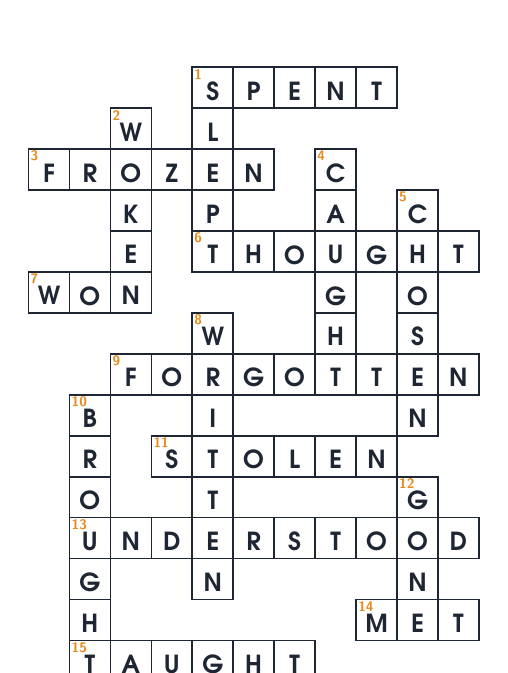
\begin{tikzpicture}[x=5.2mm,y=-5.2mm]
\fill[white] (1,11) rectangle +(1,1); \draw[ink,line width=0.6pt] (1,11) rectangle +(1,1);
\node[anchor=north west,inner sep=0.6pt,font=\uifont\bfseries\fontsize{5.5}{6}\selectfont,text=accent] at (1,11) {13};
\node[font=\hfont\bfseries\small,text=ink] at (1.5,11.58) {U};
\fill[white] (2,11) rectangle +(1,1); \draw[ink,line width=0.6pt] (2,11) rectangle +(1,1);
\node[font=\hfont\bfseries\small,text=ink] at (2.5,11.58) {N};
\fill[white] (3,11) rectangle +(1,1); \draw[ink,line width=0.6pt] (3,11) rectangle +(1,1);
\node[font=\hfont\bfseries\small,text=ink] at (3.5,11.58) {D};
\fill[white] (4,11) rectangle +(1,1); \draw[ink,line width=0.6pt] (4,11) rectangle +(1,1);
\node[font=\hfont\bfseries\small,text=ink] at (4.5,11.58) {E};
\fill[white] (5,11) rectangle +(1,1); \draw[ink,line width=0.6pt] (5,11) rectangle +(1,1);
\node[font=\hfont\bfseries\small,text=ink] at (5.5,11.58) {R};
\fill[white] (6,11) rectangle +(1,1); \draw[ink,line width=0.6pt] (6,11) rectangle +(1,1);
\node[font=\hfont\bfseries\small,text=ink] at (6.5,11.58) {S};
\fill[white] (7,11) rectangle +(1,1); \draw[ink,line width=0.6pt] (7,11) rectangle +(1,1);
\node[font=\hfont\bfseries\small,text=ink] at (7.5,11.58) {T};
\fill[white] (8,11) rectangle +(1,1); \draw[ink,line width=0.6pt] (8,11) rectangle +(1,1);
\node[font=\hfont\bfseries\small,text=ink] at (8.5,11.58) {O};
\fill[white] (9,11) rectangle +(1,1); \draw[ink,line width=0.6pt] (9,11) rectangle +(1,1);
\node[font=\hfont\bfseries\small,text=ink] at (9.5,11.58) {O};
\fill[white] (10,11) rectangle +(1,1); \draw[ink,line width=0.6pt] (10,11) rectangle +(1,1);
\node[font=\hfont\bfseries\small,text=ink] at (10.5,11.58) {D};
\fill[white] (4,6) rectangle +(1,1); \draw[ink,line width=0.6pt] (4,6) rectangle +(1,1);
\node[anchor=north west,inner sep=0.6pt,font=\uifont\bfseries\fontsize{5.5}{6}\selectfont,text=accent] at (4,6) {8};
\node[font=\hfont\bfseries\small,text=ink] at (4.5,6.58) {W};
\fill[white] (4,7) rectangle +(1,1); \draw[ink,line width=0.6pt] (4,7) rectangle +(1,1);
\node[font=\hfont\bfseries\small,text=ink] at (4.5,7.58) {R};
\fill[white] (4,8) rectangle +(1,1); \draw[ink,line width=0.6pt] (4,8) rectangle +(1,1);
\node[font=\hfont\bfseries\small,text=ink] at (4.5,8.58) {I};
\fill[white] (4,9) rectangle +(1,1); \draw[ink,line width=0.6pt] (4,9) rectangle +(1,1);
\node[font=\hfont\bfseries\small,text=ink] at (4.5,9.58) {T};
\fill[white] (4,10) rectangle +(1,1); \draw[ink,line width=0.6pt] (4,10) rectangle +(1,1);
\node[font=\hfont\bfseries\small,text=ink] at (4.5,10.58) {T};
\fill[white] (4,12) rectangle +(1,1); \draw[ink,line width=0.6pt] (4,12) rectangle +(1,1);
\node[font=\hfont\bfseries\small,text=ink] at (4.5,12.58) {N};
\fill[white] (2,7) rectangle +(1,1); \draw[ink,line width=0.6pt] (2,7) rectangle +(1,1);
\node[anchor=north west,inner sep=0.6pt,font=\uifont\bfseries\fontsize{5.5}{6}\selectfont,text=accent] at (2,7) {9};
\node[font=\hfont\bfseries\small,text=ink] at (2.5,7.58) {F};
\fill[white] (3,7) rectangle +(1,1); \draw[ink,line width=0.6pt] (3,7) rectangle +(1,1);
\node[font=\hfont\bfseries\small,text=ink] at (3.5,7.58) {O};
\fill[white] (5,7) rectangle +(1,1); \draw[ink,line width=0.6pt] (5,7) rectangle +(1,1);
\node[font=\hfont\bfseries\small,text=ink] at (5.5,7.58) {G};
\fill[white] (6,7) rectangle +(1,1); \draw[ink,line width=0.6pt] (6,7) rectangle +(1,1);
\node[font=\hfont\bfseries\small,text=ink] at (6.5,7.58) {O};
\fill[white] (7,7) rectangle +(1,1); \draw[ink,line width=0.6pt] (7,7) rectangle +(1,1);
\node[font=\hfont\bfseries\small,text=ink] at (7.5,7.58) {T};
\fill[white] (8,7) rectangle +(1,1); \draw[ink,line width=0.6pt] (8,7) rectangle +(1,1);
\node[font=\hfont\bfseries\small,text=ink] at (8.5,7.58) {T};
\fill[white] (9,7) rectangle +(1,1); \draw[ink,line width=0.6pt] (9,7) rectangle +(1,1);
\node[font=\hfont\bfseries\small,text=ink] at (9.5,7.58) {E};
\fill[white] (10,7) rectangle +(1,1); \draw[ink,line width=0.6pt] (10,7) rectangle +(1,1);
\node[font=\hfont\bfseries\small,text=ink] at (10.5,7.58) {N};
\fill[white] (1,8) rectangle +(1,1); \draw[ink,line width=0.6pt] (1,8) rectangle +(1,1);
\node[anchor=north west,inner sep=0.6pt,font=\uifont\bfseries\fontsize{5.5}{6}\selectfont,text=accent] at (1,8) {10};
\node[font=\hfont\bfseries\small,text=ink] at (1.5,8.58) {B};
\fill[white] (1,9) rectangle +(1,1); \draw[ink,line width=0.6pt] (1,9) rectangle +(1,1);
\node[font=\hfont\bfseries\small,text=ink] at (1.5,9.58) {R};
\fill[white] (1,10) rectangle +(1,1); \draw[ink,line width=0.6pt] (1,10) rectangle +(1,1);
\node[font=\hfont\bfseries\small,text=ink] at (1.5,10.58) {O};
\fill[white] (1,12) rectangle +(1,1); \draw[ink,line width=0.6pt] (1,12) rectangle +(1,1);
\node[font=\hfont\bfseries\small,text=ink] at (1.5,12.58) {G};
\fill[white] (1,13) rectangle +(1,1); \draw[ink,line width=0.6pt] (1,13) rectangle +(1,1);
\node[font=\hfont\bfseries\small,text=ink] at (1.5,13.58) {H};
\fill[white] (1,14) rectangle +(1,1); \draw[ink,line width=0.6pt] (1,14) rectangle +(1,1);
\node[anchor=north west,inner sep=0.6pt,font=\uifont\bfseries\fontsize{5.5}{6}\selectfont,text=accent] at (1,14) {15};
\node[font=\hfont\bfseries\small,text=ink] at (1.5,14.58) {T};
\fill[white] (3,9) rectangle +(1,1); \draw[ink,line width=0.6pt] (3,9) rectangle +(1,1);
\node[anchor=north west,inner sep=0.6pt,font=\uifont\bfseries\fontsize{5.5}{6}\selectfont,text=accent] at (3,9) {11};
\node[font=\hfont\bfseries\small,text=ink] at (3.5,9.58) {S};
\fill[white] (5,9) rectangle +(1,1); \draw[ink,line width=0.6pt] (5,9) rectangle +(1,1);
\node[font=\hfont\bfseries\small,text=ink] at (5.5,9.58) {O};
\fill[white] (6,9) rectangle +(1,1); \draw[ink,line width=0.6pt] (6,9) rectangle +(1,1);
\node[font=\hfont\bfseries\small,text=ink] at (6.5,9.58) {L};
\fill[white] (7,9) rectangle +(1,1); \draw[ink,line width=0.6pt] (7,9) rectangle +(1,1);
\node[font=\hfont\bfseries\small,text=ink] at (7.5,9.58) {E};
\fill[white] (8,9) rectangle +(1,1); \draw[ink,line width=0.6pt] (8,9) rectangle +(1,1);
\node[font=\hfont\bfseries\small,text=ink] at (8.5,9.58) {N};
\fill[white] (2,14) rectangle +(1,1); \draw[ink,line width=0.6pt] (2,14) rectangle +(1,1);
\node[font=\hfont\bfseries\small,text=ink] at (2.5,14.58) {A};
\fill[white] (3,14) rectangle +(1,1); \draw[ink,line width=0.6pt] (3,14) rectangle +(1,1);
\node[font=\hfont\bfseries\small,text=ink] at (3.5,14.58) {U};
\fill[white] (4,14) rectangle +(1,1); \draw[ink,line width=0.6pt] (4,14) rectangle +(1,1);
\node[font=\hfont\bfseries\small,text=ink] at (4.5,14.58) {G};
\fill[white] (5,14) rectangle +(1,1); \draw[ink,line width=0.6pt] (5,14) rectangle +(1,1);
\node[font=\hfont\bfseries\small,text=ink] at (5.5,14.58) {H};
\fill[white] (6,14) rectangle +(1,1); \draw[ink,line width=0.6pt] (6,14) rectangle +(1,1);
\node[font=\hfont\bfseries\small,text=ink] at (6.5,14.58) {T};
\fill[white] (9,3) rectangle +(1,1); \draw[ink,line width=0.6pt] (9,3) rectangle +(1,1);
\node[anchor=north west,inner sep=0.6pt,font=\uifont\bfseries\fontsize{5.5}{6}\selectfont,text=accent] at (9,3) {5};
\node[font=\hfont\bfseries\small,text=ink] at (9.5,3.58) {C};
\fill[white] (9,4) rectangle +(1,1); \draw[ink,line width=0.6pt] (9,4) rectangle +(1,1);
\node[font=\hfont\bfseries\small,text=ink] at (9.5,4.58) {H};
\fill[white] (9,5) rectangle +(1,1); \draw[ink,line width=0.6pt] (9,5) rectangle +(1,1);
\node[font=\hfont\bfseries\small,text=ink] at (9.5,5.58) {O};
\fill[white] (9,6) rectangle +(1,1); \draw[ink,line width=0.6pt] (9,6) rectangle +(1,1);
\node[font=\hfont\bfseries\small,text=ink] at (9.5,6.58) {S};
\fill[white] (9,8) rectangle +(1,1); \draw[ink,line width=0.6pt] (9,8) rectangle +(1,1);
\node[font=\hfont\bfseries\small,text=ink] at (9.5,8.58) {N};
\fill[white] (4,4) rectangle +(1,1); \draw[ink,line width=0.6pt] (4,4) rectangle +(1,1);
\node[anchor=north west,inner sep=0.6pt,font=\uifont\bfseries\fontsize{5.5}{6}\selectfont,text=accent] at (4,4) {6};
\node[font=\hfont\bfseries\small,text=ink] at (4.5,4.58) {T};
\fill[white] (5,4) rectangle +(1,1); \draw[ink,line width=0.6pt] (5,4) rectangle +(1,1);
\node[font=\hfont\bfseries\small,text=ink] at (5.5,4.58) {H};
\fill[white] (6,4) rectangle +(1,1); \draw[ink,line width=0.6pt] (6,4) rectangle +(1,1);
\node[font=\hfont\bfseries\small,text=ink] at (6.5,4.58) {O};
\fill[white] (7,4) rectangle +(1,1); \draw[ink,line width=0.6pt] (7,4) rectangle +(1,1);
\node[font=\hfont\bfseries\small,text=ink] at (7.5,4.58) {U};
\fill[white] (8,4) rectangle +(1,1); \draw[ink,line width=0.6pt] (8,4) rectangle +(1,1);
\node[font=\hfont\bfseries\small,text=ink] at (8.5,4.58) {G};
\fill[white] (10,4) rectangle +(1,1); \draw[ink,line width=0.6pt] (10,4) rectangle +(1,1);
\node[font=\hfont\bfseries\small,text=ink] at (10.5,4.58) {T};
\fill[white] (7,2) rectangle +(1,1); \draw[ink,line width=0.6pt] (7,2) rectangle +(1,1);
\node[anchor=north west,inner sep=0.6pt,font=\uifont\bfseries\fontsize{5.5}{6}\selectfont,text=accent] at (7,2) {4};
\node[font=\hfont\bfseries\small,text=ink] at (7.5,2.58) {C};
\fill[white] (7,3) rectangle +(1,1); \draw[ink,line width=0.6pt] (7,3) rectangle +(1,1);
\node[font=\hfont\bfseries\small,text=ink] at (7.5,3.58) {A};
\fill[white] (7,5) rectangle +(1,1); \draw[ink,line width=0.6pt] (7,5) rectangle +(1,1);
\node[font=\hfont\bfseries\small,text=ink] at (7.5,5.58) {G};
\fill[white] (7,6) rectangle +(1,1); \draw[ink,line width=0.6pt] (7,6) rectangle +(1,1);
\node[font=\hfont\bfseries\small,text=ink] at (7.5,6.58) {H};
\fill[white] (4,0) rectangle +(1,1); \draw[ink,line width=0.6pt] (4,0) rectangle +(1,1);
\node[anchor=north west,inner sep=0.6pt,font=\uifont\bfseries\fontsize{5.5}{6}\selectfont,text=accent] at (4,0) {1};
\node[font=\hfont\bfseries\small,text=ink] at (4.5,0.58) {S};
\fill[white] (4,1) rectangle +(1,1); \draw[ink,line width=0.6pt] (4,1) rectangle +(1,1);
\node[font=\hfont\bfseries\small,text=ink] at (4.5,1.58) {L};
\fill[white] (4,2) rectangle +(1,1); \draw[ink,line width=0.6pt] (4,2) rectangle +(1,1);
\node[font=\hfont\bfseries\small,text=ink] at (4.5,2.58) {E};
\fill[white] (4,3) rectangle +(1,1); \draw[ink,line width=0.6pt] (4,3) rectangle +(1,1);
\node[font=\hfont\bfseries\small,text=ink] at (4.5,3.58) {P};
\fill[white] (0,2) rectangle +(1,1); \draw[ink,line width=0.6pt] (0,2) rectangle +(1,1);
\node[anchor=north west,inner sep=0.6pt,font=\uifont\bfseries\fontsize{5.5}{6}\selectfont,text=accent] at (0,2) {3};
\node[font=\hfont\bfseries\small,text=ink] at (0.5,2.58) {F};
\fill[white] (1,2) rectangle +(1,1); \draw[ink,line width=0.6pt] (1,2) rectangle +(1,1);
\node[font=\hfont\bfseries\small,text=ink] at (1.5,2.58) {R};
\fill[white] (2,2) rectangle +(1,1); \draw[ink,line width=0.6pt] (2,2) rectangle +(1,1);
\node[font=\hfont\bfseries\small,text=ink] at (2.5,2.58) {O};
\fill[white] (3,2) rectangle +(1,1); \draw[ink,line width=0.6pt] (3,2) rectangle +(1,1);
\node[font=\hfont\bfseries\small,text=ink] at (3.5,2.58) {Z};
\fill[white] (5,2) rectangle +(1,1); \draw[ink,line width=0.6pt] (5,2) rectangle +(1,1);
\node[font=\hfont\bfseries\small,text=ink] at (5.5,2.58) {N};
\fill[white] (5,0) rectangle +(1,1); \draw[ink,line width=0.6pt] (5,0) rectangle +(1,1);
\node[font=\hfont\bfseries\small,text=ink] at (5.5,0.58) {P};
\fill[white] (6,0) rectangle +(1,1); \draw[ink,line width=0.6pt] (6,0) rectangle +(1,1);
\node[font=\hfont\bfseries\small,text=ink] at (6.5,0.58) {E};
\fill[white] (7,0) rectangle +(1,1); \draw[ink,line width=0.6pt] (7,0) rectangle +(1,1);
\node[font=\hfont\bfseries\small,text=ink] at (7.5,0.58) {N};
\fill[white] (8,0) rectangle +(1,1); \draw[ink,line width=0.6pt] (8,0) rectangle +(1,1);
\node[font=\hfont\bfseries\small,text=ink] at (8.5,0.58) {T};
\fill[white] (2,1) rectangle +(1,1); \draw[ink,line width=0.6pt] (2,1) rectangle +(1,1);
\node[anchor=north west,inner sep=0.6pt,font=\uifont\bfseries\fontsize{5.5}{6}\selectfont,text=accent] at (2,1) {2};
\node[font=\hfont\bfseries\small,text=ink] at (2.5,1.58) {W};
\fill[white] (2,3) rectangle +(1,1); \draw[ink,line width=0.6pt] (2,3) rectangle +(1,1);
\node[font=\hfont\bfseries\small,text=ink] at (2.5,3.58) {K};
\fill[white] (2,4) rectangle +(1,1); \draw[ink,line width=0.6pt] (2,4) rectangle +(1,1);
\node[font=\hfont\bfseries\small,text=ink] at (2.5,4.58) {E};
\fill[white] (2,5) rectangle +(1,1); \draw[ink,line width=0.6pt] (2,5) rectangle +(1,1);
\node[font=\hfont\bfseries\small,text=ink] at (2.5,5.58) {N};
\fill[white] (9,10) rectangle +(1,1); \draw[ink,line width=0.6pt] (9,10) rectangle +(1,1);
\node[anchor=north west,inner sep=0.6pt,font=\uifont\bfseries\fontsize{5.5}{6}\selectfont,text=accent] at (9,10) {12};
\node[font=\hfont\bfseries\small,text=ink] at (9.5,10.58) {G};
\fill[white] (9,12) rectangle +(1,1); \draw[ink,line width=0.6pt] (9,12) rectangle +(1,1);
\node[font=\hfont\bfseries\small,text=ink] at (9.5,12.58) {N};
\fill[white] (9,13) rectangle +(1,1); \draw[ink,line width=0.6pt] (9,13) rectangle +(1,1);
\node[font=\hfont\bfseries\small,text=ink] at (9.5,13.58) {E};
\fill[white] (0,5) rectangle +(1,1); \draw[ink,line width=0.6pt] (0,5) rectangle +(1,1);
\node[anchor=north west,inner sep=0.6pt,font=\uifont\bfseries\fontsize{5.5}{6}\selectfont,text=accent] at (0,5) {7};
\node[font=\hfont\bfseries\small,text=ink] at (0.5,5.58) {W};
\fill[white] (1,5) rectangle +(1,1); \draw[ink,line width=0.6pt] (1,5) rectangle +(1,1);
\node[font=\hfont\bfseries\small,text=ink] at (1.5,5.58) {O};
\fill[white] (8,13) rectangle +(1,1); \draw[ink,line width=0.6pt] (8,13) rectangle +(1,1);
\node[anchor=north west,inner sep=0.6pt,font=\uifont\bfseries\fontsize{5.5}{6}\selectfont,text=accent] at (8,13) {14};
\node[font=\hfont\bfseries\small,text=ink] at (8.5,13.58) {M};
\fill[white] (10,13) rectangle +(1,1); \draw[ink,line width=0.6pt] (10,13) rectangle +(1,1);
\node[font=\hfont\bfseries\small,text=ink] at (10.5,13.58) {T};
\end{tikzpicture}
\end{minipage}\hfill
\begin{minipage}[t]{0.25\linewidth}\vspace{0pt}
{\hfont\bfseries\footnotesize\color{accent}ACROSS}\par \begin{aitem}\ai{1}{\textbf{spent}}{\upillA{5}}\end{aitem}
\begin{aitem}\ai{3}{\textbf{frozen}}{\upillA{7}}\end{aitem}
\begin{aitem}\ai{6}{\textbf{thought}}{\upillA{5}\,\upillA{15}}\end{aitem}
\begin{aitem}\ai{7}{\textbf{won}}{\upillA{7}}\end{aitem}
\begin{aitem}\ai{9}{\textbf{forgotten}}{\upillA{8}}\end{aitem}
\begin{aitem}\ai{11}{\textbf{stolen}}{\upillA{7}}\end{aitem}
\begin{aitem}\ai{13}{\textbf{understood}}{\upillA{15}}\end{aitem}
\begin{aitem}\ai{14}{\textbf{met}}{\upillA{5}}\end{aitem}
\begin{aitem}\ai{15}{\textbf{taught}}{\upillA{5}}\end{aitem}
\end{minipage}\hfill
\begin{minipage}[t]{0.25\linewidth}\vspace{0pt}
{\hfont\bfseries\footnotesize\color{accent}DOWN}\par \begin{aitem}\ai{1}{\textbf{slept}}{\upillA{8}\,\upillA{12}}\end{aitem}
\begin{aitem}\ai{2}{\textbf{woken}}{\upillA{7}}\end{aitem}
\begin{aitem}\ai{4}{\textbf{caught}}{\upillA{7}}\end{aitem}
\begin{aitem}\ai{5}{\textbf{chosen}}{\upillA{7}}\end{aitem}
\begin{aitem}\ai{8}{\textbf{written}}{\upillA{7}\,\upillA{8}}\end{aitem}
\begin{aitem}\ai{10}{\textbf{brought}}{\upillA{7}}\end{aitem}
\begin{aitem}\ai{12}{\textbf{gone}}{\upillA{7}}\end{aitem}
\end{minipage}
\par\why{Past simple (finished time, a story): spent, taught, thought, met. Past participle (have/has/had + -ed/-en): all the others. Watch out for won (not winned), woken, frozen, forgotten, understood.}


\akhead{3}{Questions in the wild}{\upillA{2}\,\upillA{5}\,\upillA{6}\,\upillA{7}\,\upillA{8}\,\upillA{9}\,\upillA{11}\,\upillA{12}\,\upillA{14}\,\upillA{15}\,\upillA{17}}
\begin{multicols}{2}
\begin{aitem}\ai{1}{How long have you been back in Leuven?}{\upillA{11}}\end{aitem}
\begin{aitem}\ai{2}{Have you ever been to the Ardennes?}{\upillA{8}}\end{aitem}
\begin{aitem}\ai{3}{What have you been up to since the summer?}{\upillA{9}}\end{aitem}
\begin{aitem}\ai{4}{How often do you go to the gym?}{\upillA{2}}\end{aitem}
\begin{aitem}\ai{5}{What were you doing when the blackout happened?}{\upillA{6}}\end{aitem}
\begin{aitem}\ai{6}{Have you checked the exam timetable yet?}{\upillA{7}}\end{aitem}
\begin{aitem}\ai{7}{What time did you go to bed last night?}{\upillA{5}\,\upillA{14}}\end{aitem}
\begin{aitem}\ai{8}{Have you got a spare pen?}{\upillA{17}}\end{aitem}
\begin{aitem}\ai{9}{Had the lecture already started when you arrived?}{\upillA{15}}\end{aitem}
\begin{aitem}\ai{10}{How long have you been learning Dutch?}{\upillA{11}\,\upillA{12}}\end{aitem}
\end{multicols}
\why{be up to (something) = be doing something. ‘What have you been up to?’ is one of the most common questions when you meet someone again.}


\akhead{4}{Same words, different story}{\upillA{3}\,\upillA{4}\,\upillA{6}\,\upillA{7}\,\upillA{10}\,\upillA{14}\,\upillA{15}\,\upillA{17}}
\begin{multicols}{2}
\begin{aitem}\ai{1}{\textbf{a–i, b–ii}}{\upillA{14}}\an{have lived = I still live there; lived = a finished period.}\end{aitem}
\begin{aitem}\ai{2}{\textbf{a–ii, b–i}}{\upillA{6}\,\upillA{15}}\an{was leaving = she was in the middle of leaving; had left = she had gone before I arrived.}\end{aitem}
\begin{aitem}\ai{3}{\textbf{a–i, b–ii}}{\upillA{10}}\an{been fixing = the activity (maybe not finished); fixed = the result.}\end{aitem}
\begin{aitem}\ai{4}{\textbf{a–ii, b–i}}{\upillA{3}}\an{always + continuous = too often, with irritation.}\end{aitem}
\begin{aitem}\ai{5}{\textbf{a–ii, b–i}}{\upillA{4}}\an{think of (opinion) = simple; thinking about (mental activity now) = continuous.}\end{aitem}
\begin{aitem}\ai{6}{\textbf{a–i, b–ii}}{\upillA{4}}\an{is = his character; is being = his behaviour right now.}\end{aitem}
\begin{aitem}\ai{7}{\textbf{a–ii, b–i}}{\upillA{6}}\an{had dinner = after the call; was having dinner = it had already started.}\end{aitem}
\begin{aitem}\ai{8}{\textbf{a–i, b–ii}}{\upillA{7}}\an{gone = he’s there now; been = he went and came back.}\end{aitem}
\begin{aitem}\ai{9}{\textbf{a–ii, b–i}}{\upillA{15}}\an{had logged off = before the match ended.}\end{aitem}
\begin{aitem}\ai{10}{\textbf{a–i, b–ii}}{\upillA{17}}\an{having = an event/action happening now; have = possession.}\end{aitem}
\begin{aitem}\ai{11}{\textbf{a–ii, b–i}}{\upillA{14}}\an{haven’t seen = the morning isn’t over; didn’t see = the morning is finished.}\end{aitem}
\end{multicols}


\akhead{5}{One situation, two angles}{\upillA{9}\,\upillA{10}\,\upillA{11}\,\upillA{12}\,\upillA{17}}\begin{aitem}\ai{1}{I’ve been revising for the thermodynamics exam since 9 a.m.\newline I’ve covered four chapters.}{\upillA{9}\,\upillA{10}\,\upillA{12}}\end{aitem}
\begin{aitem}\ai{2}{Wout has been playing ranked all evening.\newline He’s lost six games in a row.}{\upillA{10}}\end{aitem}
\begin{aitem}\ai{3}{We’ve been trying to fix this bug for two hours.\newline We’ve found three new bugs.}{\upillA{10}\,\upillA{12}}\end{aitem}
\begin{aitem}\ai{4}{My housemate has been cooking since lunchtime.\newline She’s / He’s made enough lasagne for ten people.}{\upillA{10}}\end{aitem}
\begin{aitem}\ai{5}{I’ve had this laptop since 2021. (not have been having)\newline It’s crashed three times this week.}{\upillA{10}\,\upillA{11}\,\upillA{17}}\end{aitem}
\begin{aitem}\ai{6}{I’ve been learning Dutch for two years.\newline I’ve learnt (learned) about 2,000 words.}{\upillA{10}\,\upillA{12}}\end{aitem}
\begin{aitem}\ai{7}{Ines and I have known each other since primary school. (not have been knowing)\newline She’s visited me in Leuven twice.}{\upillA{10}\,\upillA{11}}\end{aitem}
\begin{aitem}\ai{8}{I’ve been training for a half-marathon since September.\newline I’ve run over 300 km.}{\upillA{10}\,\upillA{12}}\end{aitem}
\why{Traps: \emph{have} (possession) and \emph{know} are state verbs, so they stay simple even with for/since: I’ve had…, we’ve known…}


\akhead{6}{The Monday from hell}{\upillA{5}\,\upillA{6}\,\upillA{15}\,\upillA{16}}\begin{aitem}\ai{1}{Because his phone had died / his phone’s battery had run out (at 6:50).}{\upillA{15}}\an{Earlier past \arr{} past perfect.}\end{aitem}
\begin{aitem}\ai{2}{He’d been playing Overwatch with his friends (for three hours).}{\upillA{16}}\end{aitem}
\begin{aitem}\ai{3}{He was looking for his student card.}{\upillA{6}}\end{aitem}
\begin{aitem}\ai{4}{His (bike) chain came off.}{\upillA{5}\,\upillA{6}}\an{A short action in the middle of a longer one \arr{} past simple.}\end{aitem}
\begin{aitem}\ai{5}{Yes, it had (already) started — seven minutes earlier.}{\upillA{15}}\end{aitem}
\begin{aitem}\ai{6}{Because he’d been running (for about twenty minutes).}{\upillA{16}}\end{aitem}
\begin{aitem}\ai{7}{They’d been writing for seven minutes.}{\upillA{16}}\end{aitem}
\ai{8}{\emph{Model:} When Tiago finally walked into the exam hall, the other students had already been writing for seven minutes. He was out of breath because he’d been running since his bike chain came off. He’d overslept: his phone had died during the night, so his alarm hadn’t gone off. While the invigilator was finding him a seat, he was still trying to calm down. In the end, the exam went well — not bad for a Monday from hell!}{\upillA{5}\,\upillA{6}\,\upillA{15}\,\upillA{16}}


\akhead{7}{Continuous allowed?}{\upillA{4}\,\upillA{17}}
\begin{multicols}{2}
\begin{aitem}\ai{1}{\textcolor{good}{\ding{51}} — think of/about = consider, so the continuous is fine.}{\upillA{4}}\end{aitem}
\begin{aitem}\ai{2}{\textcolor{bad}{\ding{55}} \arr{} I don’t understand. (understand is a state verb; ‘I’m not understanding’ is heard informally, but avoid it.)}{\upillA{4}}\end{aitem}
\begin{aitem}\ai{3}{\textcolor{bad}{\ding{55}} \arr{} it needs}{\upillA{4}}\end{aitem}
\begin{aitem}\ai{4}{\textcolor{good}{\ding{51}} — for how someone looks or feels now, simple and continuous are both fine.}{\upillA{4}}\end{aitem}
\begin{aitem}\ai{5}{\textcolor{good}{\ding{51}} — have = experience/enjoy (an action), not possession.}{\upillA{17}}\end{aitem}
\begin{aitem}\ai{6}{\textcolor{bad}{\ding{55}} \arr{} has / has got (possession)}{\upillA{17}}\end{aitem}
\begin{aitem}\ai{7}{\textcolor{good}{\ding{51}} — is being = is behaving (right now).}{\upillA{4}}\end{aitem}
\begin{aitem}\ai{8}{\textcolor{bad}{\ding{55}} \arr{} don’t belong}{\upillA{4}}\end{aitem}
\begin{aitem}\ai{9}{\textcolor{bad}{\ding{55}} \arr{} Do you see / Can you see}{\upillA{4}}\end{aitem}
\begin{aitem}\ai{10}{\textcolor{good}{\ding{51}} — How are you feeling? = How do you feel?}{\upillA{4}}\end{aitem}
\begin{aitem}\ai{11}{\textcolor{bad}{\ding{55}} \arr{} I usually feel (a general habit)}{\upillA{4}}\end{aitem}
\begin{aitem}\ai{12}{\textcolor{bad}{\ding{55}} \arr{} What do you think of…? (opinion)}{\upillA{4}}\end{aitem}
\end{multicols}


\akhead{8}{Micro-dialogues}{\upillA{5}\,\upillA{6}\,\upillA{7}\,\upillA{8}\,\upillA{11}\,\upillA{12}\,\upillA{13}\,\upillA{14}\,\upillA{17}}
\begin{multicols}{2}
\begin{aitem}\ai{1}{\textbf{has stolen} {\color{inksoft}/ ’s stolen}}{\upillA{7}\,\upillA{13}}\end{aitem}
\begin{aitem}\ai{2}{\textbf{did it happen}}{\upillA{13}\,\upillA{14}}\an{The news is in the present perfect; the details (when?) go into the past simple.}\end{aitem}
\begin{aitem}\ai{3}{\textbf{noticed}}{\upillA{13}\,\upillA{14}}\end{aitem}
\begin{aitem}\ai{4}{\textbf{’s gone} {\color{inksoft}/ has gone}}{\upillA{7}}\an{He’s there now. AmE also: He went to the workshop.}\end{aitem}
\begin{aitem}\ai{5}{\textbf{Have you ever tried}}{\upillA{8}}\end{aitem}
\begin{aitem}\ai{6}{\textbf{had}}{\upillA{13}\,\upillA{14}}\end{aitem}
\begin{aitem}\ai{7}{\textbf{was}}{\upillA{14}}\end{aitem}
\begin{aitem}\ai{8}{\textbf{haven’t slept}}{\upillA{8}\,\upillA{12}}\end{aitem}
\begin{aitem}\ai{9}{\textbf{started}}{\upillA{12}}\end{aitem}
\begin{aitem}\ai{10}{\textbf{have you known}}{\upillA{11}}\end{aitem}
\begin{aitem}\ai{11}{\textbf{met}}{\upillA{5}\,\upillA{12}}\end{aitem}
\begin{aitem}\ai{12}{\textbf{spilled} {\color{inksoft}/ spilt}}{\upillA{5}}\end{aitem}
\begin{aitem}\ai{13}{\textbf{’ve cut} {\color{inksoft}/ have cut}}{\upillA{7}\,\upillA{13}}\end{aitem}
\begin{aitem}\ai{14}{\textbf{did you do}}{\upillA{13}}\end{aitem}
\begin{aitem}\ai{15}{\textbf{was stripping}}{\upillA{6}}\end{aitem}
\begin{aitem}\ai{16}{\textbf{slipped}}{\upillA{6}}\end{aitem}
\begin{aitem}\ai{17}{\textbf{Did you see}}{\upillA{14}}\end{aitem}
\begin{aitem}\ai{18}{\textbf{didn’t have}}{\upillA{17}}\end{aitem}
\begin{aitem}\ai{19}{\textbf{was working} {\color{inksoft}/ worked}}{\upillA{6}}\an{was working stresses the activity in progress while the match was on; worked is also fine.}\end{aitem}
\begin{aitem}\ai{20}{\textbf{went}}{\upillA{12}}\end{aitem}
\begin{aitem}\ai{21}{\textbf{haven’t been}}{\upillA{8}\,\upillA{12}}\end{aitem}
\begin{aitem}\ai{22}{\textbf{has broken}}{\upillA{8}}\an{That’s the third time… + present perfect.}\end{aitem}
\begin{aitem}\ai{23}{\textbf{’ve brought} {\color{inksoft}/ have brought / brought}}{\upillA{7}\,\upillA{8}}\an{today isn’t finished, so the present perfect is the safe choice in BrE; brought is also common.}\end{aitem}
\end{multicols}


\akhead{9}{Voice chat: Thursday, 22:47}{\upillA{1}\,\upillA{3}\,\upillA{4}\,\upillA{5}\,\upillA{6}\,\upillA{7}\,\upillA{8}\,\upillA{9}\,\upillA{12}\,\upillA{13}\,\upillA{14}\,\upillA{15}\,\upillA{17}}
\begin{multicols}{2}
\begin{aitem}\ai{1}{\textbf{’ve just changed} {\color{inksoft}/ have just changed}}{\upillA{7}}\an{AmE also: I just changed.}\end{aitem}
\begin{aitem}\ai{2}{\textbf{’re breaking up} {\color{inksoft}/ are breaking up}}{\upillA{1}}\end{aitem}
\begin{aitem}\ai{3}{\textbf{’s been spiking} {\color{inksoft}/ has been spiking}}{\upillA{9}}\end{aitem}
\begin{aitem}\ai{4}{\textbf{’s downloading} {\color{inksoft}/ is downloading / ’s been downloading}}{\upillA{1}}\an{happening now; ’s been downloading (all evening) also works.}\end{aitem}
\begin{aitem}\ai{5}{\textbf{’s playing} {\color{inksoft}/ is playing}}{\upillA{1}}\an{this game, right now — not in general.}\end{aitem}
\begin{aitem}\ai{6}{\textbf{haven’t played}}{\upillA{8}\,\upillA{12}}\end{aitem}
\begin{aitem}\ai{7}{\textbf{lost}}{\upillA{14}}\end{aitem}
\begin{aitem}\ai{8}{\textbf{’s flanking} {\color{inksoft}/ is flanking}}{\upillA{1}}\end{aitem}
\begin{aitem}\ai{9}{\textbf{do you see} {\color{inksoft}/ can you see}}{\upillA{4}}\end{aitem}
\begin{aitem}\ai{10}{\textbf{has} {\color{inksoft}/ ’s got / has got}}{\upillA{17}}\end{aitem}
\begin{aitem}\ai{11}{\textbf{’ve been farming} {\color{inksoft}/ have been farming}}{\upillA{9}}\end{aitem}
\begin{aitem}\ai{12}{\textbf{shot} {\color{inksoft}/ ’s shot / has shot}}{\upillA{5}\,\upillA{13}}\an{recent news: past simple or present perfect (Unit 13B) — in fast comms the past simple is more common.}\end{aitem}
\begin{aitem}\ai{13}{\textbf{’s killed} {\color{inksoft}/ has killed}}{\upillA{8}}\end{aitem}
\begin{aitem}\ai{14}{\textbf{’s always doing} {\color{inksoft}/ is always doing}}{\upillA{3}}\an{always + continuous = it happens too often (and it’s annoying).}\end{aitem}
\begin{aitem}\ai{15}{\textbf{was holding}}{\upillA{6}}\end{aitem}
\begin{aitem}\ai{16}{\textbf{bombed}}{\upillA{6}}\end{aitem}
\begin{aitem}\ai{17}{\textbf{got}}{\upillA{15}}\end{aitem}
\begin{aitem}\ai{18}{\textbf{’d already taken} {\color{inksoft}/ had already taken}}{\upillA{15}}\end{aitem}
\begin{aitem}\ai{19}{\textbf{’ve been fighting} {\color{inksoft}/ have been fighting}}{\upillA{9}}\end{aitem}
\begin{aitem}\ai{20}{\textbf{still haven’t won}}{\upillA{7}}\end{aitem}
\begin{aitem}\ai{21}{\textbf{think}}{\upillA{4}}\an{think = believe/have an opinion \arr{} simple.}\end{aitem}
\begin{aitem}\ai{22}{\textbf{have you got} {\color{inksoft}/ do you have}}{\upillA{17}}\end{aitem}
\begin{aitem}\ai{23}{\textbf{’ve got} {\color{inksoft}/ have}}{\upillA{17}}\end{aitem}
\begin{aitem}\ai{24}{\textbf{haven’t even started}}{\upillA{7}}\end{aitem}
\end{multicols}
\why{Phrasebook:} \enspace 1\,c \enspace 2\,g \enspace 3\,e \enspace 4\,f \enspace 5\,b \enspace 6\,h \enspace 7\,a \enspace 8\,d


\akhead{10}{Group chat: find the ten mistakes}{\upillA{4}\,\upillA{5}\,\upillA{6}\,\upillA{7}\,\upillA{8}\,\upillA{9}\,\upillA{10}\,\upillA{11}\,\upillA{12}\,\upillA{14}\,\upillA{15}\,\upillA{17}}
\why{Correct messages: 3, 4, 7 and 13.}
\begin{multicols}{2}
\begin{aitem}\ai{1}{msg 1: I \textbf{finished} the wiring diagram yesterday}{\upillA{14}}\an{finished time (yesterday) \arr{} past simple}\end{aitem}
\begin{aitem}\ai{2}{msg 2: I\textbf{’ve been working} on the PID code since Monday}{\upillA{9}\,\upillA{11}}\an{since Monday \arr{} present perfect (continuous)}\end{aitem}
\begin{aitem}\ai{5}{msg 5: I \textbf{know} a guy…}{\upillA{4}}\an{know is a state verb}\end{aitem}
\begin{aitem}\ai{6}{msg 6: the left sensor \textbf{hasn’t worked / hasn’t been working} since…}{\upillA{11}\,\upillA{12}}\an{since + a point in the past \arr{} present perfect}\end{aitem}
\begin{aitem}\ai{8}{msg 8: when \textbf{did you send} the draft…?}{\upillA{12}\,\upillA{14}}\an{When…? asks for a finished time \arr{} past simple}\end{aitem}
\begin{aitem}\ai{9}{msg 9: I \textbf{was sleeping}}{\upillA{6}}\an{in the middle of sleeping when the call came}\end{aitem}
\begin{aitem}\ai{10}{msg 10: It’s the first time I\textbf{’ve used} an oscilloscope}{\upillA{8}}\an{It’s the first time + present perfect}\end{aitem}
\begin{aitem}\ai{11}{msg 11: we \textbf{had} a meeting with our supervisor last Tuesday}{\upillA{17}}\an{past of have (got) = had}\end{aitem}
\begin{aitem}\ai{12}{msg 12: Lien \textbf{has written} six pages}{\upillA{10}}\an{how much/how many \arr{} present perfect simple}\end{aitem}
\begin{aitem}\ai{14}{msg 14: by the time I got to the lab, everyone \textbf{had left}}{\upillA{15}}\an{they left before I arrived}\end{aitem}
\end{multicols}
\why{Vault words: \emph{wrap your head around something} = manage to understand something difficult; \emph{chip away at something} = make progress little by little.}


\akhead{11}{The case of the flooded kot}{\upillA{5}\,\upillA{6}\,\upillA{7}\,\upillA{8}\,\upillA{9}\,\upillA{11}\,\upillA{13}\,\upillA{15}\,\upillA{16}}
{\hfont\bfseries\footnotesize\color{cDaily}A}\par
\begin{multicols}{2}
\begin{aitem}\ai{1}{\textbf{’ve just arrived} {\color{inksoft}/ have just arrived}}{\upillA{7}}\an{AmE also: I just arrived.}\end{aitem}
\begin{aitem}\ai{2}{\textbf{has the water been coming}}{\upillA{9}\,\upillA{11}}\end{aitem}
\begin{aitem}\ai{3}{\textbf{’s been} {\color{inksoft}/ has been}}{\upillA{11}}\an{be + for weeks, from then until now \arr{} present perfect.}\end{aitem}
\begin{aitem}\ai{4}{\textbf{’ve told} {\color{inksoft}/ have told}}{\upillA{7}\,\upillA{8}}\end{aitem}
\begin{aitem}\ai{5}{\textbf{’ve called} {\color{inksoft}/ have called / called}}{\upillA{7}\,\upillA{13}}\an{new information with a result now (a plumber is coming); called is also possible.}\end{aitem}
\end{multicols}
{\hfont\bfseries\footnotesize\color{cDaily}B}\par
\begin{aitem}\ai{a}{Bram — he was going into the bathroom.}{\upillA{6}}\end{aitem}
\begin{aitem}\ai{b}{No. She’d had a shower the night before and went straight downstairs.}{\upillA{15}}\end{aitem}
\begin{aitem}\ai{c}{Downstairs — she had already gone down.}{\upillA{15}}\end{aitem}
\begin{aitem}\ai{d}{He was (still) sleeping.}{\upillA{6}}\end{aitem}
\begin{aitem}\ai{e}{Bram. He shaved after his shower, and nobody used the bathroom after him.}{\upillA{5}}\end{aitem}
\ai{f}{\emph{Model:} It wasn’t Chloé: she had already gone downstairs when Bram came out of the bathroom, and she never went back up. It wasn’t Dries either: when he got up, everyone had already left and the water was already coming under the door.}{\upillA{15}}
\why{What the tenses tell you: Bram \emph{was going into} the bathroom when Ana came out of her room, so Ana used the kitchen. Chloé \emph{had already gone} downstairs when Bram came out, and she never went back up. Dries was asleep until everyone \emph{had left} — and by then the water \emph{was already coming} under the door. So the last person at the sink was Bram, who shaved after his shower. Case closed.}


\akhead{12}{Email to your professor}{\upillA{7}\,\upillA{8}\,\upillA{9}\,\upillA{10}\,\upillA{12}\,\upillA{14}\,\upillA{15}}
\begin{multicols}{3}
\begin{aitem}\ai{1}{\textbf{have} {\color{inksoft}/ ’ve}}{\upillA{9}}\end{aitem}
\begin{aitem}\ai{2}{\textbf{since}}{\upillA{12}}\end{aitem}
\begin{aitem}\ai{3}{\textbf{just} {\color{inksoft}/ recently}}{\upillA{7}\,\upillA{8}}\end{aitem}
\begin{aitem}\ai{4}{\textbf{ago}}{\upillA{12}\,\upillA{14}}\end{aitem}
\begin{aitem}\ai{5}{\textbf{had}}{\upillA{15}}\end{aitem}
\begin{aitem}\ai{6}{\textbf{haven’t}}{\upillA{7}}\end{aitem}
\begin{aitem}\ai{7}{\textbf{yet}}{\upillA{7}}\end{aitem}
\begin{aitem}\ai{8}{\textbf{has}}{\upillA{9}\,\upillA{10}}\end{aitem}
\begin{aitem}\ai{9}{\textbf{for}}{\upillA{12}}\end{aitem}
\begin{aitem}\ai{10}{\textbf{ever}}{\upillA{8}}\end{aitem}
\begin{aitem}\ai{11}{\textbf{Have}}{\upillA{7}\,\upillA{8}}\an{‘Did you had…’ is impossible, so only Have fits.}\end{aitem}
\begin{aitem}\ai{12}{\textbf{haven’t}}{\upillA{8}}\end{aitem}
\end{multicols}


\akhead{13}{Sherlock mode}{\upillA{9}\,\upillA{10}\,\upillA{16}}
\begin{multicols}{2}
\begin{aitem}\ai{1}{He’s been fixing / repairing his bike.}{\upillA{9}}\end{aitem}
\begin{aitem}\ai{2}{He’s been shouting (callouts) all night.}{\upillA{9}}\end{aitem}
\begin{aitem}\ai{3}{Someone has been soldering (and has burnt something).}{\upillA{9}\,\upillA{10}}\end{aitem}
\begin{aitem}\ai{4}{I’ve been studying (or gaming!) all night.}{\upillA{9}}\end{aitem}
\begin{aitem}\ai{5}{Someone has eaten all the stroopwafels! (finished result \arr{} simple)}{\upillA{10}}\end{aitem}
\begin{aitem}\ai{6}{It’s been raining (hard) / He’s been walking in the rain.}{\upillA{9}}\end{aitem}
\begin{aitem}\ai{7}{He’s been grinding ranked / playing a lot of ranked.}{\upillA{9}}\end{aitem}
\begin{aitem}\ai{8}{She’d been doing yoga / working out.}{\upillA{16}}\end{aitem}
\begin{aitem}\ai{9}{They’d been drawing (cartoons of) him on the whiteboard.}{\upillA{16}}\end{aitem}
\end{multicols}
\why{Other verbs are fine if the logic works (e.g. card 2: He’s been yelling; card 4: You’ve been revising). The key point is the form: have/has been -ing (cards 1–4, 6–7), have/has + past participle for a finished result (card 5), had been -ing for the past cards (8–9).}


\akhead{14}{Same meaning, new shape}{\upillA{7}\,\upillA{8}\,\upillA{9}\,\upillA{11}\,\upillA{12}\,\upillA{14}\,\upillA{15}\,\upillA{17}}
\begin{multicols}{2}
\begin{aitem}\ai{1}{\textbf{have been studying}}{\upillA{11}\,\upillA{12}}\end{aitem}
\begin{aitem}\ai{2}{\textbf{haven’t visited my grandparents since}}{\upillA{11}\,\upillA{12}}\end{aitem}
\begin{aitem}\ai{3}{\textbf{the best fries}}{\upillA{8}}\end{aitem}
\begin{aitem}\ai{4}{\textbf{I’ve used}}{\upillA{8}}\end{aitem}
\begin{aitem}\ai{5}{\textbf{have known Arne}}{\upillA{11}}\end{aitem}
\begin{aitem}\ai{6}{\textbf{haven’t been to the cinema for}}{\upillA{12}}\end{aitem}
\begin{aitem}\ai{7}{\textbf{How long have you been}}{\upillA{12}}\end{aitem}
\begin{aitem}\ai{8}{\textbf{has gone to}}{\upillA{7}}\end{aitem}
\begin{aitem}\ai{9}{\textbf{had already started}}{\upillA{15}}\end{aitem}
\begin{aitem}\ai{10}{\textbf{Have you got}}{\upillA{17}}\end{aitem}
\begin{aitem}\ai{11}{\textbf{lived in São Paulo for}}{\upillA{14}}\an{Trap: 2015–2022 is a finished period, so it’s past simple — not have lived.}\end{aitem}
\begin{aitem}\ai{12}{\textbf{has been playing for}}{\upillA{9}\,\upillA{12}}\end{aitem}
\end{multicols}


\akhead{15}{The 3-second rule}{\upillA{3}\,\upillA{4}\,\upillA{6}\,\upillA{7}\,\upillA{8}\,\upillA{9}\,\upillA{11}\,\upillA{12}\,\upillA{15}\,\upillA{16}\,\upillA{17}}
\begin{multicols}{2}
\begin{aitem}\ai{1}{I’ve lived / I’ve been living in Leuven for three years.}{\upillA{11}}\an{há/faz + present in Portuguese \arr{} present perfect + for in English.}\end{aitem}
\begin{aitem}\ai{2}{I haven’t played with you guys for ages! / It’s been ages since I played with you!}{\upillA{11}\,\upillA{12}}\end{aitem}
\begin{aitem}\ai{3}{I’ve just woken up — give me five minutes.}{\upillA{7}}\an{acabar de = have just (AmE also: I just woke up).}\end{aitem}
\begin{aitem}\ai{4}{Have you ever been to Bruges?}{\upillA{8}}\an{já (experience) = ever; foi a = been to.}\end{aitem}
\begin{aitem}\ai{5}{How long have you been playing support?}{\upillA{11}\,\upillA{12}}\an{Not ‘Since when do you play…?’}\end{aitem}
\begin{aitem}\ai{6}{When I arrived, the lecture/class had already started.}{\upillA{15}}\end{aitem}
\begin{aitem}\ai{7}{I was playing when the internet went down.}{\upillA{6}}\end{aitem}
\begin{aitem}\ai{8}{It’s the first time I’ve eaten / had waterzooi.}{\upillA{8}}\an{Not ‘the first time I eat’.}\end{aitem}
\begin{aitem}\ai{9}{He’s always leaving the dishes in the sink.}{\upillA{3}}\an{viver + -ndo (annoying habit) = always + continuous.}\end{aitem}
\begin{aitem}\ai{10}{I’ve got a headache. / I have a headache.}{\upillA{17}}\an{estar com (illness) = have (got).}\end{aitem}
\begin{aitem}\ai{11}{I’ve known her since first year.}{\upillA{11}}\end{aitem}
\begin{aitem}\ai{12}{We’d been waiting for twenty minutes when the bus finally came.}{\upillA{16}}\end{aitem}
\begin{aitem}\ai{13}{What do you think of the course? / How are you finding the course?}{\upillA{4}}\an{Opinion \arr{} think (simple). ‘How are you finding…?’ is a natural alternative.}\end{aitem}
\begin{aitem}\ai{14}{It’s been raining since yesterday.}{\upillA{9}\,\upillA{12}}\an{Not ‘It’s raining since yesterday’.}\end{aitem}
\end{multicols}


\akhead{16}{Rapid fire}{\upillA{1}\,\upillA{2}\,\upillA{3}\,\upillA{6}\,\upillA{8}\,\upillA{9}\,\upillA{11}\,\upillA{12}\,\upillA{13}\,\upillA{15}\,\upillA{17}}
\why{There’s no single right answer — these are models to compare with yours. Did your first verb have the right tense? Did you keep it when you added details?}
\begin{multicols}{2}
\begin{aitem}\ai{1}{\emph{At the moment I’m working on our Engineering Experience project — we’re building a robot. I’m also writing a lab report.}}{\upillA{1}}\end{aitem}
\begin{aitem}\ai{2}{\emph{I usually go for a run after class, and in the evening I play a few games with friends on Discord.}}{\upillA{2}}\end{aitem}
\begin{aitem}\ai{3}{\emph{I’ve been reading out loud, watching series without subtitles and talking to classmates as much as I can.}}{\upillA{9}}\end{aitem}
\begin{aitem}\ai{4}{\emph{Yes, I have — once, before a physics exam. I studied until five, slept for two hours and almost missed the bus.}}{\upillA{8}\,\upillA{13}}\end{aitem}
\begin{aitem}\ai{5}{\emph{This time last year I was still living in Brazil and studying for my exams there.}}{\upillA{6}}\end{aitem}
\begin{aitem}\ai{6}{\emph{The best match I’ve ever played was a comeback in overtime: we were losing, but we won the last three fights.}}{\upillA{8}\,\upillA{13}}\end{aitem}
\begin{aitem}\ai{7}{\emph{I’ve known my oldest friend since primary school. We met because the teacher made us sit together.}}{\upillA{11}\,\upillA{12}}\end{aitem}
\begin{aitem}\ai{8}{\emph{Before I moved to Belgium, I’d never cycled in the rain every day — or eaten fries with mayonnaise!}}{\upillA{15}}\end{aitem}
\begin{aitem}\ai{9}{\emph{My teammate is always forgetting to unmute himself, so we spend half the match shouting ‘You’re muted!’}}{\upillA{3}}\end{aitem}
\begin{aitem}\ai{10}{\emph{I’ve got my laptop, a charger, two notebooks and a half-eaten sandwich.}}{\upillA{17}}\end{aitem}
\end{multicols}


\akhead{17}{One story, three speeds}{\upillA{5}\,\upillA{6}\,\upillA{8}\,\upillA{13}\,\upillA{15}\,\upillA{16}}
\why{A model for story C (about 2 minutes at a relaxed pace). The target forms are in bold.}\par
\begin{tcolorbox}[enhanced,colback=paper,colframe=paper,arc=1.5mm,fontupper=\small,left=3mm,right=3mm]
It \textbf{was} a Tuesday afternoon, and we \textbf{were doing} our first electronics lab. Everybody \textbf{was rushing} because the session ended at five. I\textbf{’d never used} that kind of power supply before, and I\textbf{’d been staring} at the circuit diagram for twenty minutes without really understanding it. My lab partner \textbf{connected} the last capacitor, and I \textbf{switched} on the power. Suddenly there \textbf{was} a loud pop and a lot of smoke. We\textbf{’d connected} the capacitor the wrong way round! The TA \textbf{ran} over, \textbf{switched} everything off and \textbf{looked} at us in silence. It \textbf{was} the first time I\textbf{’d} ever \textbf{burnt} a component. Since then, I\textbf{’ve checked} every circuit twice before switching it on — and I \textbf{haven’t burnt} anything else. Yet.
\end{tcolorbox}


\akhead{18}{Shadow \& rebuild}{\upillA{1}\,\upillA{2}\,\upillA{5}\,\upillA{6}\,\upillA{7}\,\upillA{8}\,\upillA{9}\,\upillA{15}\,\upillA{16}}
\why{No key needed — but check your rebuilt version for these: \emph{I’ve been back… for} (not \emph{I’m back since}) \mdot{}\ \emph{I’d been using} (before another past moment) \mdot{}\ \emph{I was ordering… and I froze} (background + event) \mdot{}\ \emph{I’d forgotten} \mdot{}\ \emph{I’ve already had} (this week isn’t over). Vault: \emph{dust something off} = start using a skill again after a long time.}



\vspace{4mm}
\begin{infobox}{UNIT TAGS}
\begin{multicols}{3}\small\RaggedRight
\textbf{U1}\enspace Present continuous\par
\textbf{U2}\enspace Present simple\par
\textbf{U3}\enspace Present cont. vs simple 1\par
\textbf{U4}\enspace Present cont. vs simple 2\par
\textbf{U5}\enspace Past simple\par
\textbf{U6}\enspace Past continuous\par
\textbf{U7}\enspace Present perfect 1\par
\textbf{U8}\enspace Present perfect 2\par
\textbf{U9}\enspace Present perfect continuous\par
\textbf{U10}\enspace Pres. perf. cont. vs simple\par
\textbf{U11}\enspace How long have you (been)…?\par
\textbf{U12}\enspace for / since; when…? / how long…?\par
\textbf{U13}\enspace Present perfect vs past 1\par
\textbf{U14}\enspace Present perfect vs past 2\par
\textbf{U15}\enspace Past perfect\par
\textbf{U16}\enspace Past perfect continuous\par
\textbf{U17}\enspace have and have got\par
\end{multicols}
\end{infobox}

\end{document}
